\subsection{Client}
Das Frontend besitzt das Design-Muster View-Model-Controler als übergeordnetes Muster. Im Packet "View" befinden sich die mit HTML und CSS designten Webseiten. Das Packet "Model" dient als Bindeglied zwischen dem "View"-Packet und dem "Controler"-Paket. Es beinhaltet die Daten die in den Aufbau einer Webseite eingebunden werden und fragt diese an und lässt sie ändern im Packet "Controler". Einen austausch zwischen dem Frontend und dem Backendserver erfolgt im Packet "Controler". Dies beinhaltet die Daten-, Lösch und Änderungsanfragen.

\begin{figure}[H]
\centerline{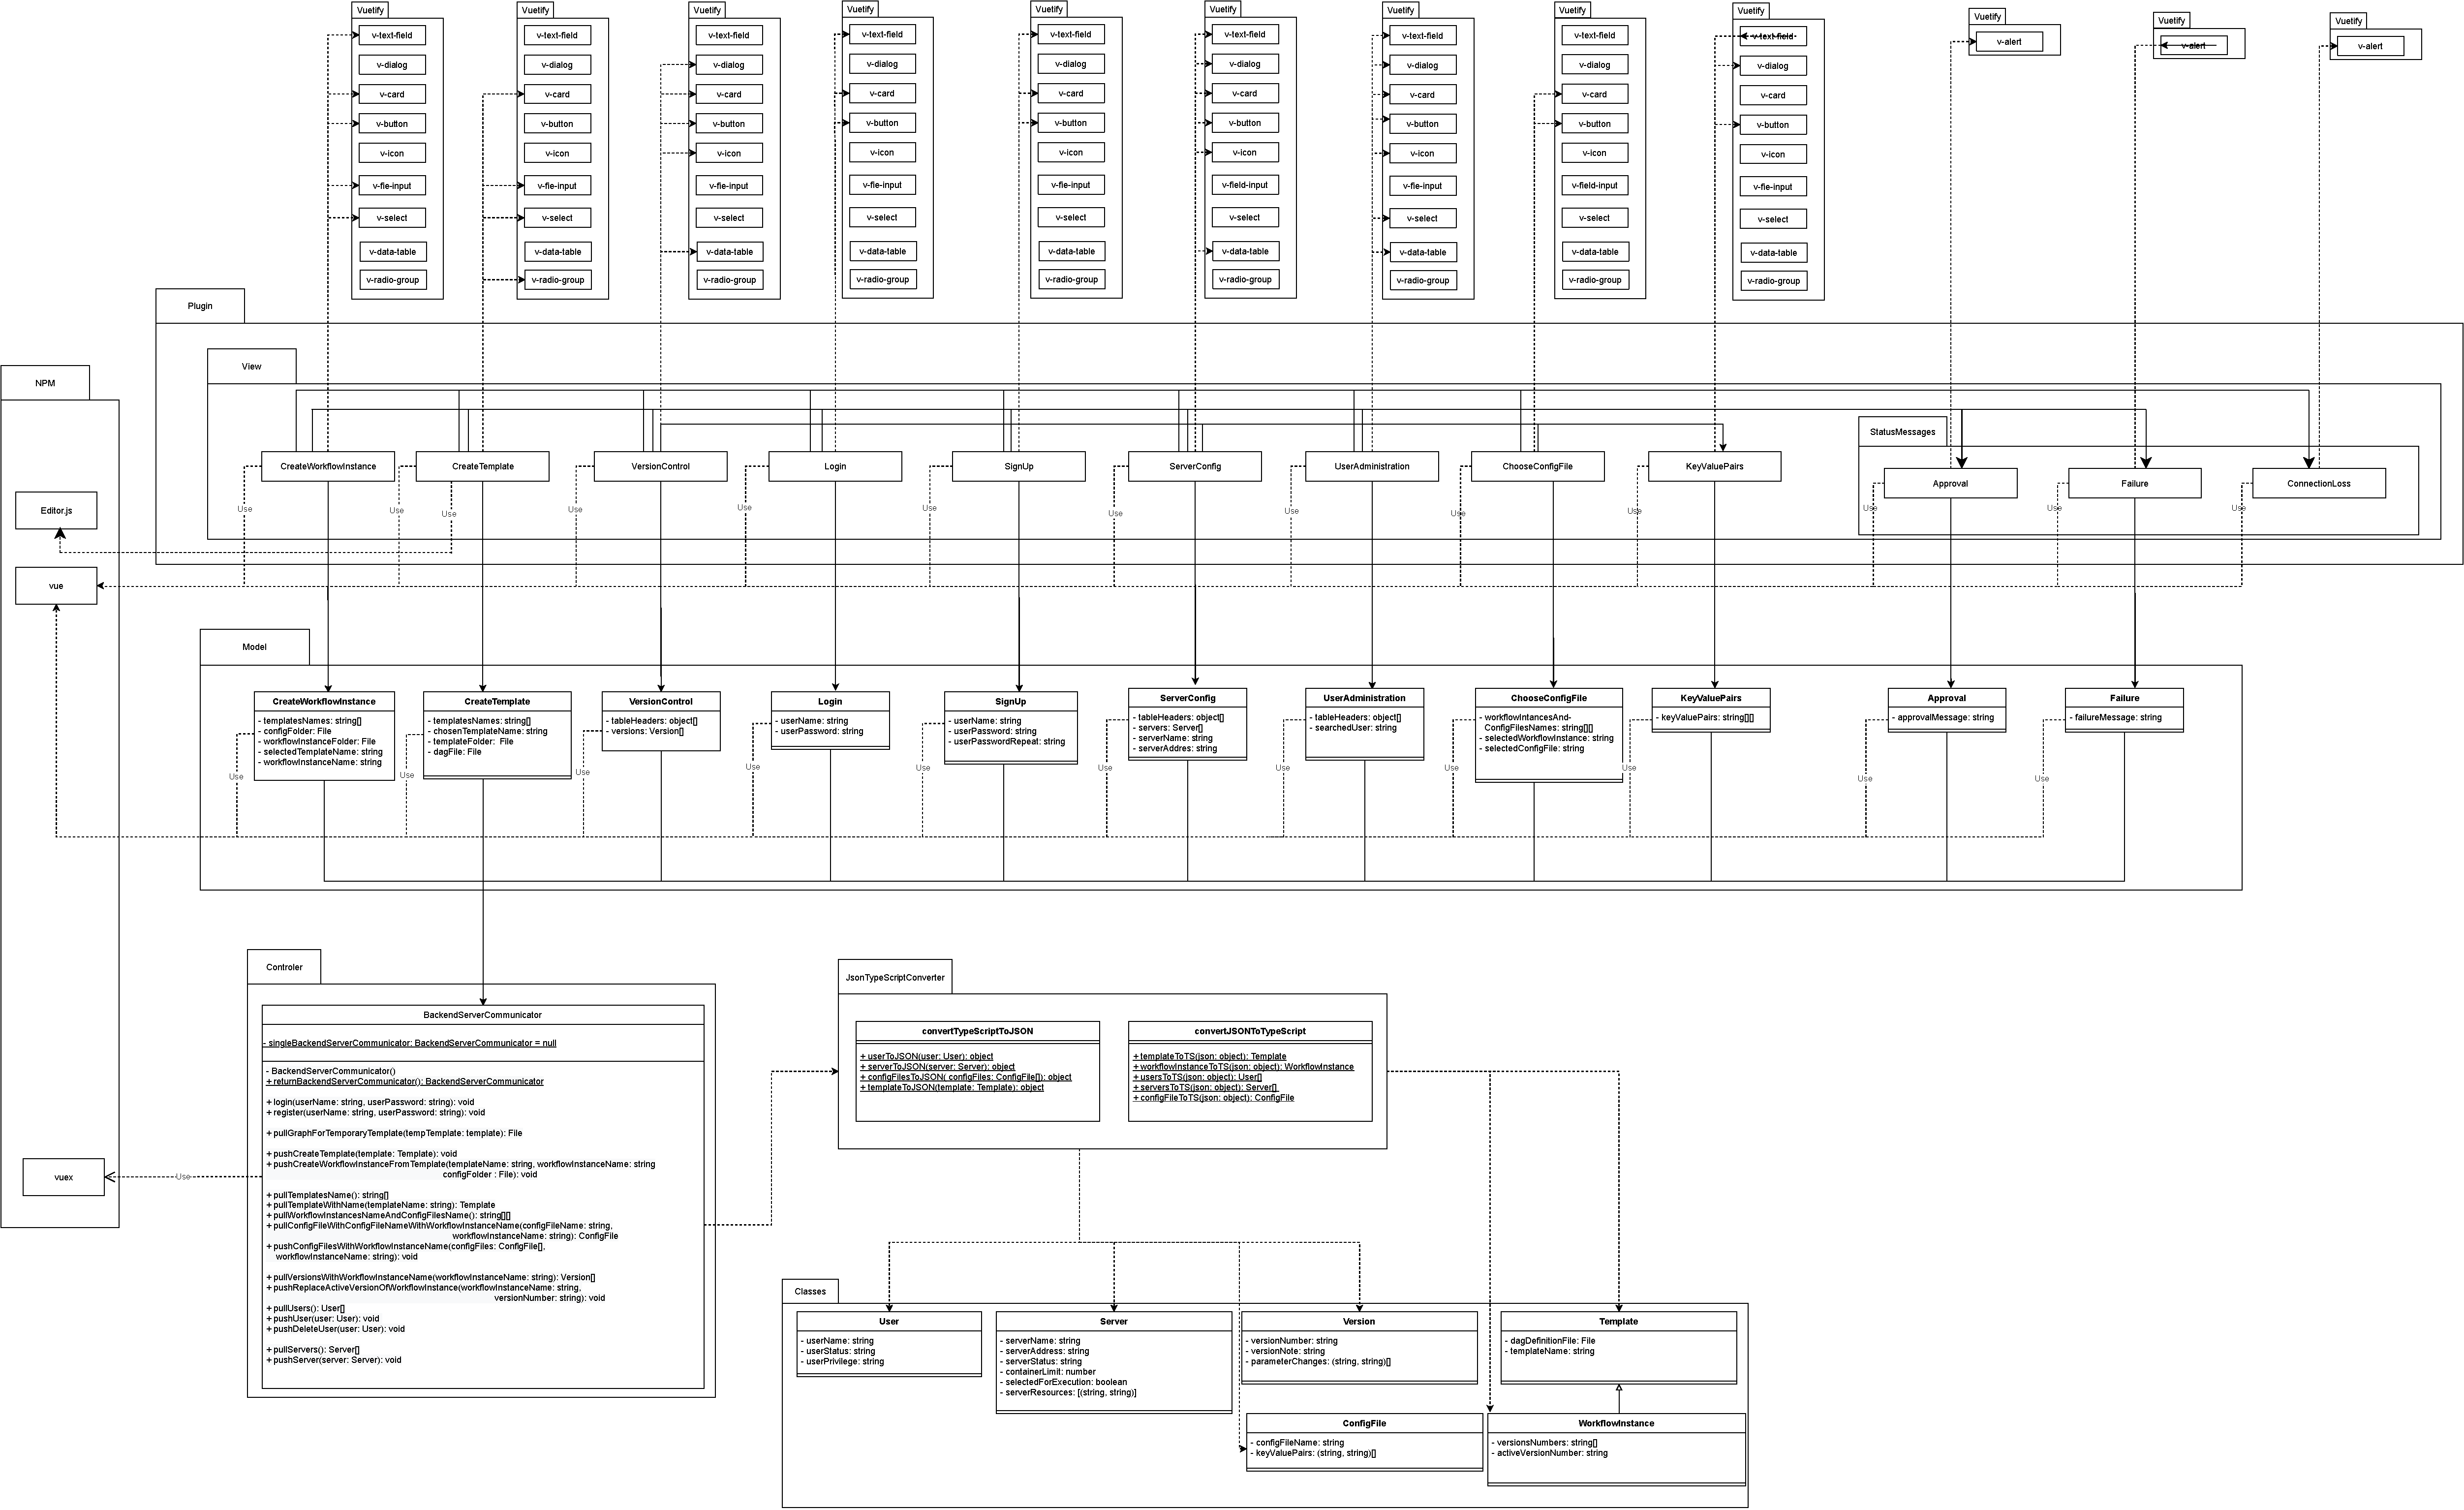
\includegraphics[scale=0.2]{res/FrontendUML.drawio.pdf}}
\caption{Klassendiagramm zum Frontend}
\end{figure}

\newpage